% Options here are passed to the article class.
% Most common options: 10pt, 11pt, 12pt
\documentclass[10pt]{datasheet}

% Input encoding and typographical rules for English language
\usepackage[utf8]{inputenc}
\usepackage[english]{babel}
\usepackage[english]{isodate}

% tikz is used to draw images in this example, but you can
% also use \includegraphics{}.
\usepackage{graphicx}

% These define global texts that are used in headers and titles.
\title{BV01: Simple Hopperspeed Grouper}
\author{Andrews54757}
\tags{box-variable, hopperspeed}
\date{October 2022}
\revision{Revision 1}

\begin{document}
\maketitle

\section{Features}

\begin{itemize}
\item{Hopperspeed with 16gt output type switching delay}
\item{Contains 9 1wt tileable svars}
\item{132 buffer slots per slice}
\end{itemize}

\section{Applications}

\begin{itemize}
\item{Optimizing box merging}
\item{Reducing Encoder Usage}
\end{itemize}

\section{General Description}
A simple hopper speed box grouper using svars. Given an input of varying boxes, it will buffer boxes with the same type to be outputted in a group when requested. Useful for reducing encoder calls. 

Has 9 svar slices with two double chests of buffer for each type. Easily expandable. Hopperlocking not included.

% Switch to next column
\vfill\break

\begin{figure}[h]
    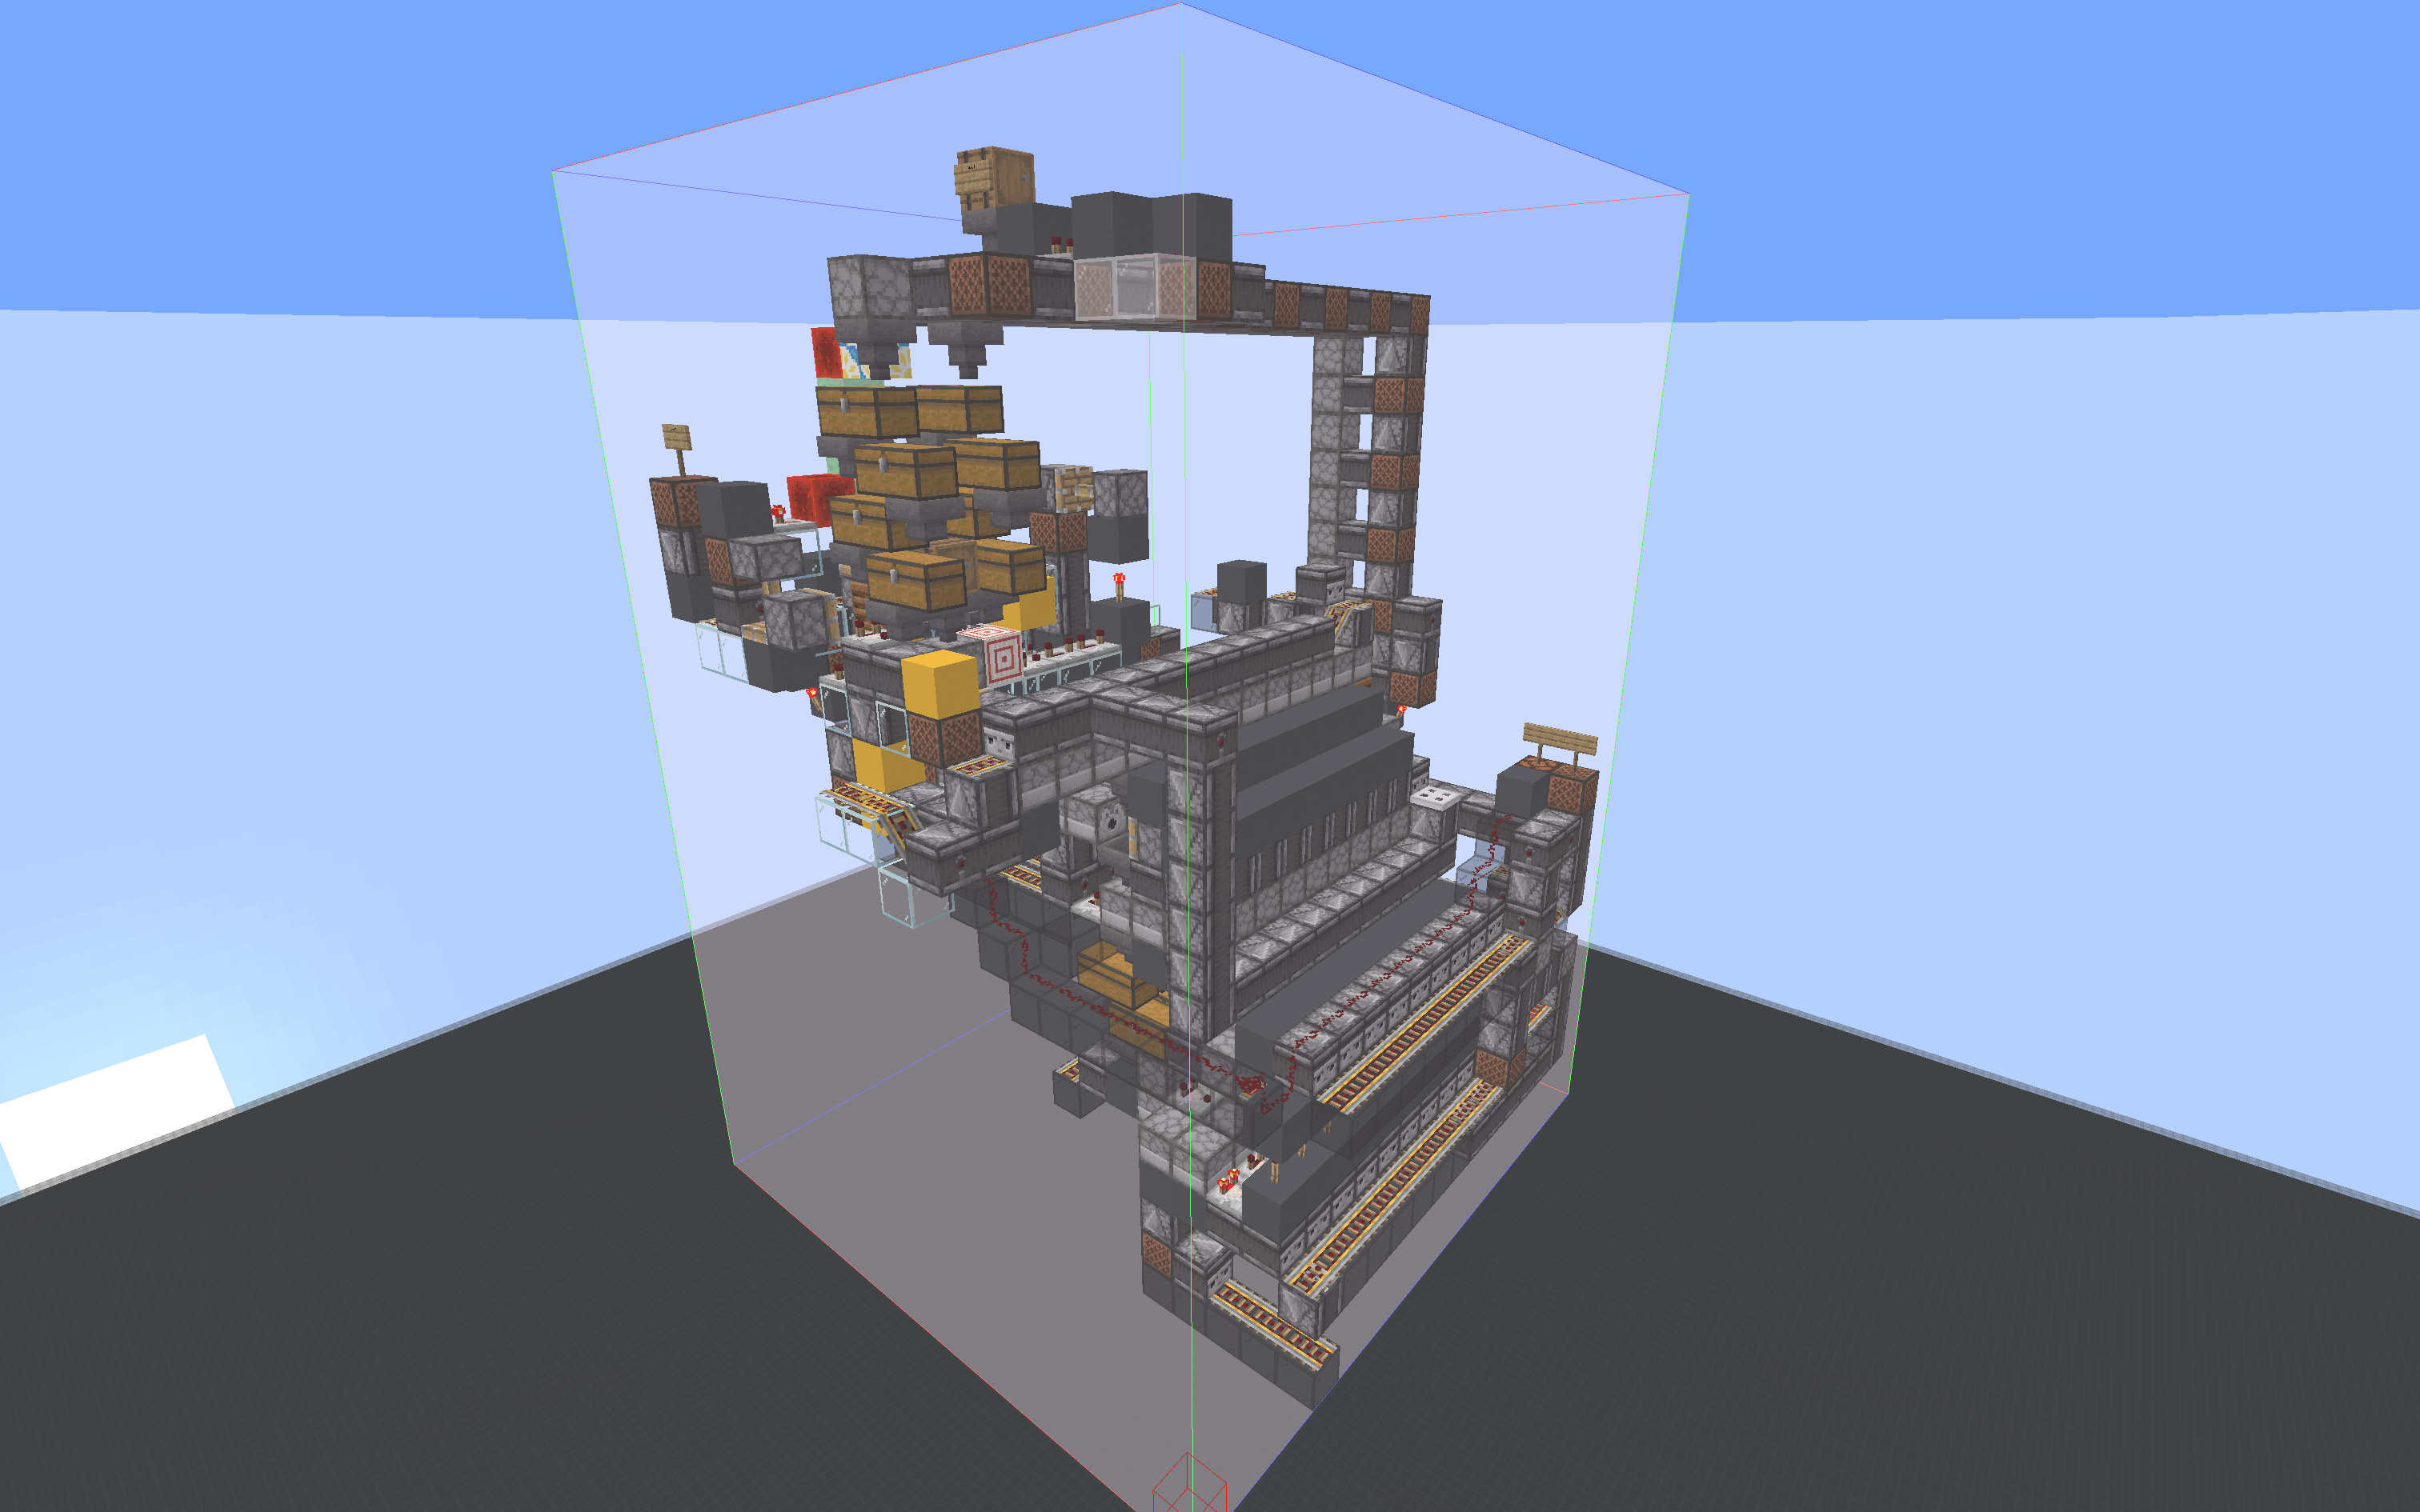
\includegraphics[width=0.5\textwidth]{grouper.png}
    \caption{Screenshot of Grouper Device}
\end{figure}

% For wide tables, a single column layout is better. It can be switched
% page-by-page.
\onecolumn

\section{Device Specifications}
All specifications are in ideal conditions at 20TPS.

\begin{table}[h]
\caption{Device Specifications}
\begin{tabularx}{\textwidth}{l | c c c | c | X}
    \thickhline
    \textbf{Parameter} & \textbf{Min.} & \textbf{Typ.} & \textbf{Max.} &
    \textbf{Unit} & \textbf{Conditions} \\
    \hline
    Input Throughput  & - & - & 1 & HS & \multirow{3}{*}{Normal Usage} \\
    Output Throughput  & - & - & 1 & HS & \\
    Switching Delay & 16 & - & - & gt & \\
    \hline
    MC Version & 1.16 & 1.17.1 & - & MCV & Latest version at time of writing: 1.19.2\\
    \hline
    Dimensions & & 17 x 18 x 28 & & Blks & \\
    \thickhline
\end{tabularx}
\end{table}

\section{Testing Data}
\begin{table}[h]
\caption{Executed Tests}
\begin{tabularx}{\textwidth}{X | X}
    \thickhline
    \textbf{Test} & \textbf{Result} \\
    \hline
    Input/output test & Device successfully grouped boxes of 12 different item types and sequentlially outputted them in hopperspeed\\
    \thickhline
\end{tabularx}
\end{table}

\section{Download Information}
\begin{table}[h]
    \caption{Download Information}
    \begin{tabularx}{\textwidth}{l | l | l | X}
        \thickhline
        \textbf{Identifier} & \textbf{MC} & \textbf{File} & \textbf{Description} \\
        \hline
        BV01 & 1.17.1 & \href{https://github.com/Soontech-Annals/Archive/blob/364bde8dbcbc2e5337489ff435bcda9b387017e2/Archive/box-variable/BV01\%20Simple\%20Hopperspeed\%20Grouper/BV01\_hopperspeed\_grouper\_p1.litematic?raw=1}{BV01\_hopperspeed\_grouper\_p1.litematic} & Litematic of grouper device \\
        \thickhline
    \end{tabularx}
\end{table}

\end{document}
